
\documentclass[tikz]{standalone}
\usepackage{graphicx}
\usepackage{lmodern}
\usepackage{amsmath, amssymb, amsfonts}
\usetikzlibrary{calc}
\newcommand{\R}{\mathcal{R}}

\begin{document}

%geometrically calc original top k
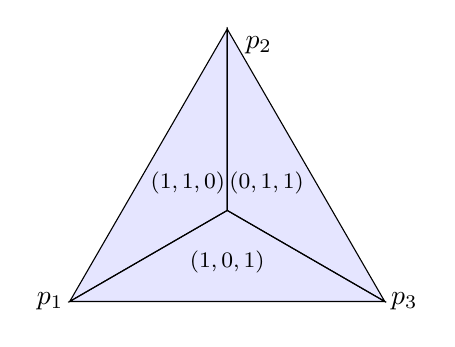
\begin{tikzpicture}
\path[fill=blue, opacity = 0.1] (2,0) -- (-2,0) -- (0,3.46) -- cycle;
%label outcomes
\node at (-9/4, 0) {$p_1$};
\node at (2/5, 3.25) {$p_2$};
\node at (9/4, 0) {$p_3$};
%level sets
\draw (2,0) -- (0, 2/1.73) -- (-2,0) -- cycle; \node at (0, 0.5) {\footnotesize$(1,0,1)$};
\draw (2,0) -- (0, 2/1.73) -- (0,3.46) -- cycle;
\node at (-1/2, 3/2) {\footnotesize$(1,1,0)$};
\draw (0,3.46) -- (0, 2/1.73) -- (-2,0) -- cycle;
\node at (1/2, 3/2) {\footnotesize$(0,1,1)$};
\end{tikzpicture}

%geometrically calculated surrogate
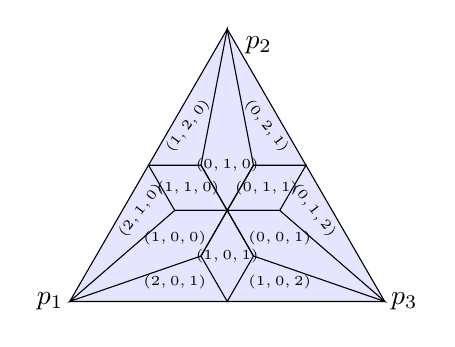
\begin{tikzpicture}
\draw[fill=blue, fill opacity = 0.1] (2,0) -- (-2,0) -- (0,3.46) -- cycle;
%label outcomes
\node at (-9/4, 0) {$p_1$};
\node at (2/5, 3.25) {$p_2$};
\node at (9/4, 0) {$p_3$};

%level sets
%kites
\draw (-2,0) -- (-1/3, 0.577) -- (0,2/1.73) -- (-2/3, 2/1.73) -- cycle; 
\draw (2,0) -- (1/3, 0.577) -- (0,2/1.73) -- (2/3, 2/1.73) -- cycle; 
\draw (0,2 * 1.73) -- (-1/3, 1.73) -- (0,2/1.73) -- (1/3, 1.73) -- cycle; 

%diamonds
\draw (0,0) -- (-1/3, 0.577) -- (0,2/1.73) -- (1/3, 0.577) -- cycle; 
\draw (-1, 1.73) -- (-2/3, 2/1.73) -- (0,2/1.73) -- (-1/3, 1.73) -- cycle; 
\draw (1, 1.73) -- (2/3, 2/1.73) -- (0,2/1.73) -- (1/3, 1.73) -- cycle; 


%nodes
\node at (0, 0.577){\fontsize{3}{12}\selectfont  $(1,0,1)$};
\node at (-2/3, 1/4){\fontsize{3}{12}\selectfont $(2,0,1)$};
\node at (2/3, 1/4){\fontsize{3}{12}\selectfont $(1,0,2)$};
\node at (-2/3, 0.577 * 1.4){\fontsize{3}{12}\selectfont $(1,0,0)$};
\node at (2/3, 1.4*0.577){\fontsize{3}{12}\selectfont $(0,0,1)$};
\node[rotate=52.5] at (-1.1, 2/1.73){\fontsize{3}{12}\selectfont $(2,1,0)$};
\node[rotate=-52.5] at (1.1, 2/1.73){\fontsize{3}{12}\selectfont $(0,1,2)$};
\node at (-1/2, 1.443){\fontsize{3}{12}\selectfont $(1,1,0)$};
\node at (1/2, 1.443){\fontsize{3}{12}\selectfont $(0,1,1)$};
\node at (0,1.73) {\fontsize{3}{12}\selectfont$(0,1,0)$};
\node[rotate=-52.5] at (1/2, 1.73 + 1/2) {\fontsize{3}{12}\selectfont$(0,2,1)$};
\node[rotate=52.5] at (-1/2, 1.73 + 1/2) {\fontsize{3}{12}\selectfont$(1,2,0)$};
\end{tikzpicture}

%OG
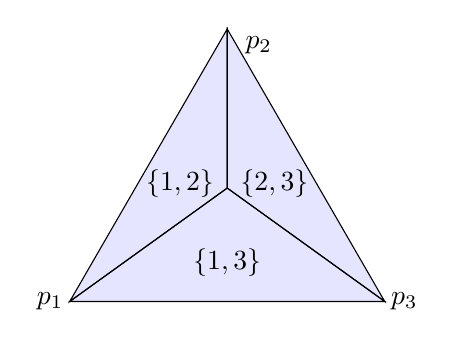
\begin{tikzpicture}
\path[fill=blue, opacity = 0.1] (2,0) -- (-2,0) -- (0,3.46) -- cycle;
%label outcomes
\node at (-9/4, 0) {$p_1$};
\node at (2/5, 3.25) {$p_2$};
\node at (9/4, 0) {$p_3$};
%level sets
\draw (2,0) -- (0, 1.44) -- (-2,0) -- cycle; \node at (0, 0.5) {$\{1,3\}$};
\draw (2,0) -- (0, 1.44) -- (0,3.46) -- cycle;
\node at (-3/5, 3/2) {$\{1,2\}$};
\draw (0,3.46) -- (0, 1.44) -- (-2,0) -- cycle;
\node at (3/5, 3/2) {$\{2,3\}$};
\end{tikzpicture}


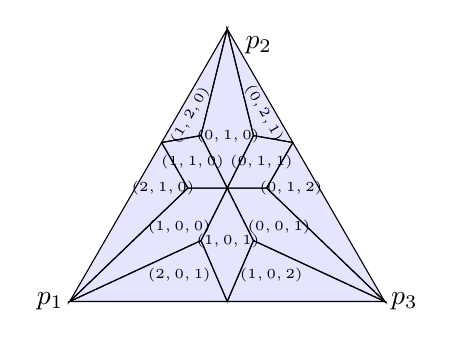
\begin{tikzpicture}
\path[fill=blue, opacity = 0.1] (2,0) -- (-2,0) -- (0,3.46) -- cycle;
%label outcomes
\node at (-9/4, 0) {$p_1$};
\node at (2/5, 3.25) {$p_2$};
\node at (9/4, 0) {$p_3$};

%level sets
%kites
\draw (-2,0) -- (-1/3, 1.44-2/3) -- (0,1.44) -- (- 1/2, 1.44) -- cycle; 
\draw (2,0) -- (1/3, 1.44 - 2/3) -- (0,1.44) -- ( 1/2, 1.44) -- cycle;
\draw (0, 3.46) -- (-1/3, 1.44 + 2/3) -- (0,1.44) -- (1/3, 1.44 + 2/3) -- cycle;

%diamonds
\draw (0,0) -- (-1/3, 1.44-2/3) -- (0,1.44) -- (1/3, 1.44-2/3) -- cycle; 
\draw (-5/6,7 * 3.46/12) -- (-1/2, 1.44) -- (0,1.44) -- (-1/3, 1.44+2/3) -- cycle; 
\draw (5/6,7 * 3.46/12) -- (1/2, 1.44) -- (0,1.44) -- (1/3, 1.44+2/3) -- cycle; 

%triangles
\draw (-2,0) -- (-5/6,7 * 3.46/12) -- (-1/2, 1.44) -- cycle; 
\draw (2,0) -- (5/6,7 * 3.46/12) -- (1/2, 1.44) --cycle; 
\draw (0,3.46) -- (-5/6,7 * 3.46/12) -- (-1/3, 1.44+2/3)  -- cycle; 
\draw (0,3.46) -- (5/6,7 * 3.46/12) -- (1/3, 1.44+2/3) -- cycle; 
\draw (-2,0) -- (-1/3, 1.44-2/3) -- (0,0) -- cycle;
\draw (2,0) -- (1/3, 1.44-2/3) -- (0,0) -- cycle;

%nodes
\node at (-0.05, 1.44-2/3){\fontsize{3}{12} \selectfont  $(1,0,1)$};
\node at (-2/3, 0.33){\fontsize{3}{12} \selectfont $(2,0,1)$};
\node at (1/2, 0.33){\fontsize{3}{12} \selectfont $(1,0,2)$};
\node at (-2/3, 1.44-1/2){\fontsize{3}{12} \selectfont $(1,0,0)$};
\node at (3/5, 1.44-1/2){\fontsize{3}{12} \selectfont $(0,0,1)$};
\node at (-7/8, 1.44){\fontsize{3}{12} \selectfont $(2,1,0)$};
\node at (3/4, 1.44){\fontsize{3}{12} \selectfont $(0,1,2)$};
\node at (-1/2, 1.44 + 1/3){\fontsize{3}{12} \selectfont $(1,1,0)$};
\node at (3/8, 1.44 + 1/3){\fontsize{3}{12} \selectfont $(0,1,1)$};
\node at (-0.05, 1.44 + 2/3) {\fontsize{3}{12} \selectfont $(0,1,0)$};
\node[rotate=-60] at (7/16, 1.44 + 1) {\fontsize{3}{12} \selectfont $(0,2,1)$};
\node[rotate=60] at (-1/2, 1.44 + 7/8) {\fontsize{3}{12} \selectfont $(1,2,0)$};
\end{tikzpicture}


\end{document}
%%% Local Variables:
%%% mode: latex
%%% TeX-master: t
%%% End:
